\documentclass{standalone}
\usepackage{pgfplots}
\pgfplotsset{compat=newest}

\begin{document}
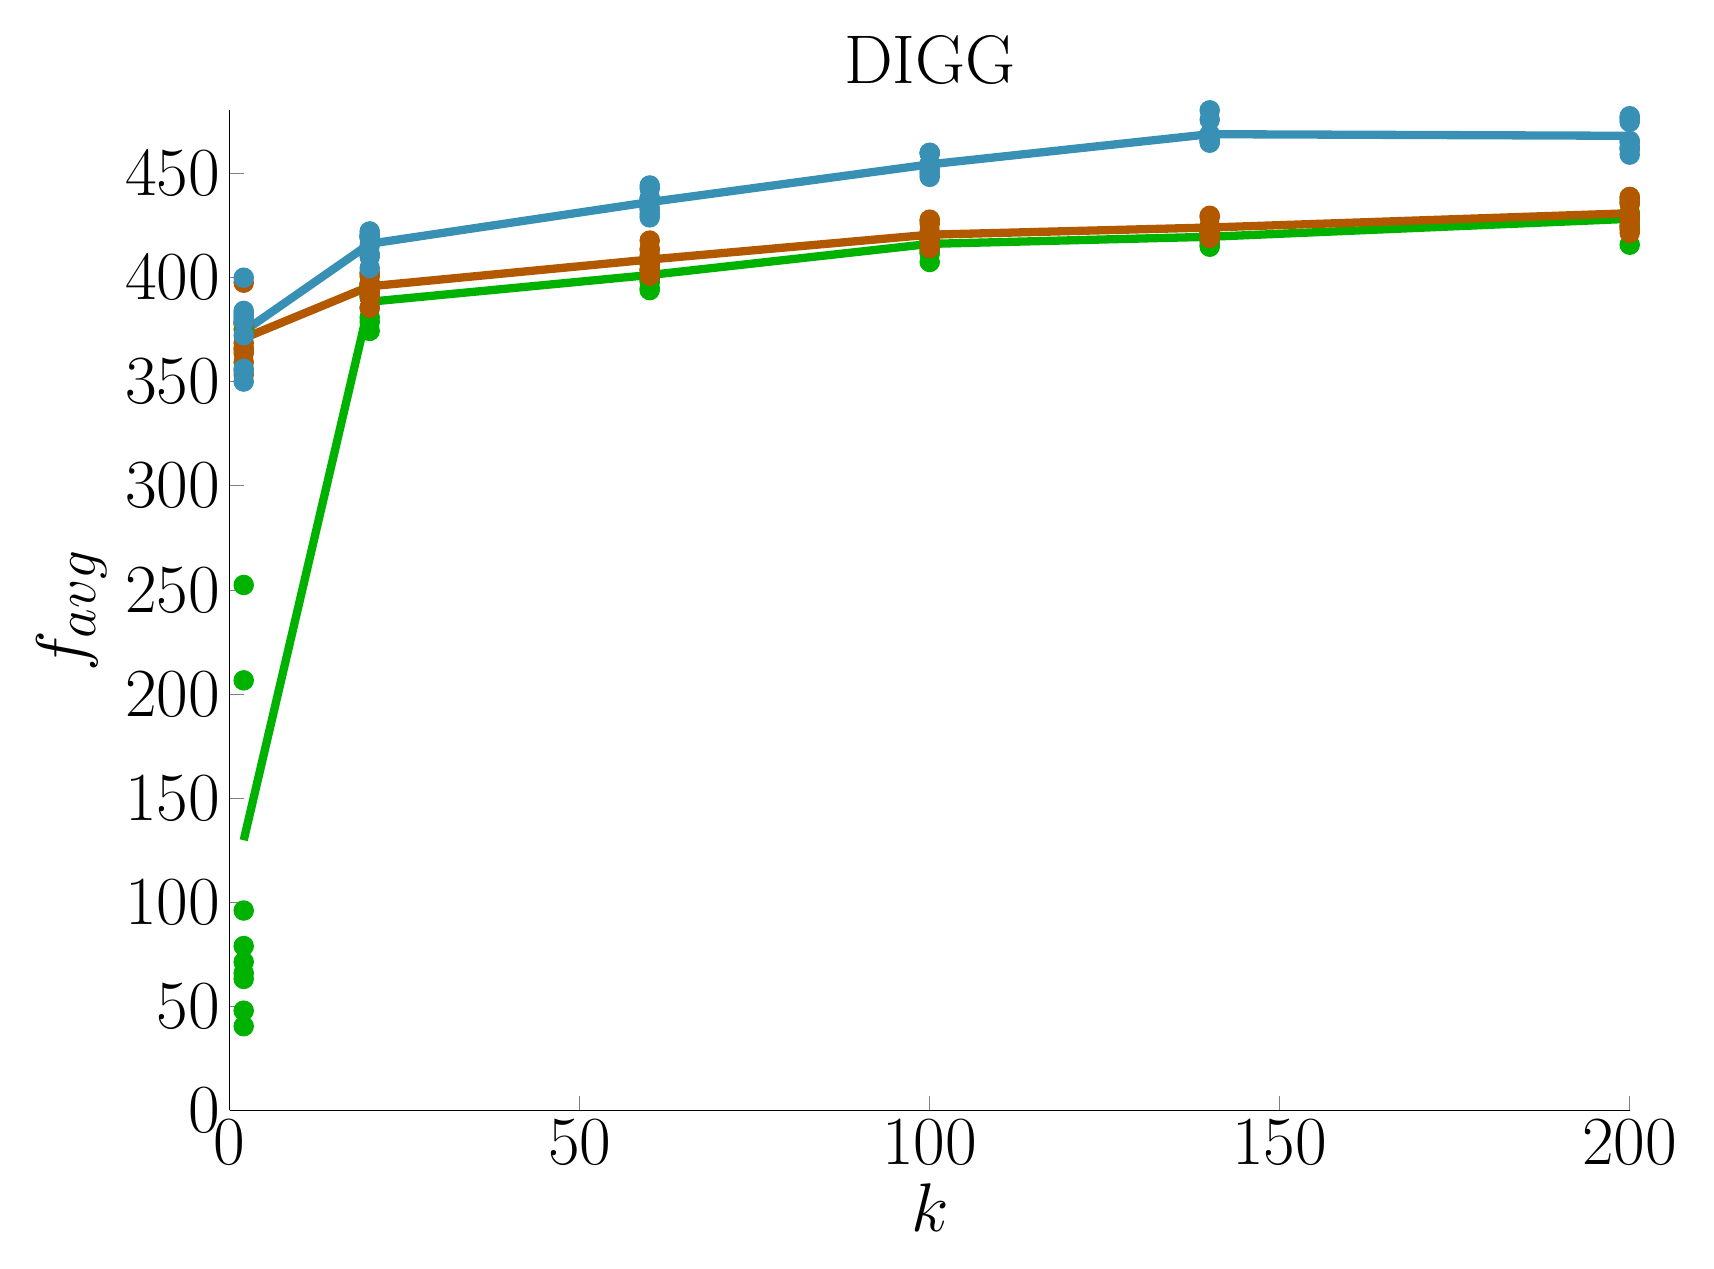
\begin{tikzpicture}

\begin{axis}[%
title style={font=\Huge},
title=DIGG,
tick label style={font=\Huge},
label style={font=\Huge},
legend style={font=\Huge},
view={0}{90},
max space between ticks=50pt,
width=7in,
height=5in,
scale only axis,
xmin=0, xmax=200,
xtick={0, 50, 100, 150, 200},
xlabel={$k$},
ymin=0, ymax=480.333333333,
ylabel={$f_{avg}$},
major tick length=5pt,
axis lines*=left,
legend cell align=left,
clip=false]

\addplot [
only marks,
mark=*,
mark size=3.5pt,
color=green!70!black,
%solid,
%line width=2pt,
]
coordinates{
(2,40.4)(2,47.8666666667)(2,63.1)(2,65.8666666667)(2,71.2666666667)(2,78.9)(2,95.9666666667)(2,206.533333333)(2,252.333333333)(2,375.0)(20,374.366666667)(20,378.633333333)(20,380.866666667)(20,385.5)(20,390.9)(20,391.8)(20,392.9)(20,395.8)(20,396.066666667)(20,397.0)(60,393.966666667)(60,394.866666667)(60,397.966666667)(60,398.466666667)(60,399.766666667)(60,400.266666667)(60,404.0)(60,406.733333333)(60,407.066666667)(60,409.133333333)(100,407.466666667)(100,411.7)(100,412.0)(100,413.033333333)(100,414.066666667)(100,417.866666667)(100,418.833333333)(100,419.566666667)(100,419.766666667)(100,427.4)(140,414.8)(140,415.7)(140,417.266666667)(140,419.133333333)(140,420.0)(140,420.033333333)(140,421.333333333)(140,422.0)(140,422.0)(140,423.566666667)(200,415.766666667)(200,423.066666667)(200,424.533333333)(200,424.966666667)(200,428.033333333)(200,429.433333333)(200,430.5)(200,431.066666667)(200,436.233333333)(200,438.6)
};

\addplot [
only marks,
mark=*,
mark size=3.5pt,
color=orange!70!black,
%solid,
%line width=2pt,
]
coordinates{
(2,353.333333333)(2,359.266666667)(2,363.666666667)(2,365.3)(2,366.233333333)(2,368.633333333)(2,377.7)(2,378.066666667)(2,378.566666667)(2,397.533333333)(20,385.433333333)(20,390.366666667)(20,392.766666667)(20,394.4)(20,396.433333333)(20,396.566666667)(20,397.1)(20,400.533333333)(20,402.0)(20,402.266666667)(60,400.866666667)(60,403.5)(60,403.733333333)(60,406.233333333)(60,408.033333333)(60,408.733333333)(60,410.766666667)(60,413.333333333)(60,413.633333333)(60,417.766666667)(100,414.166666667)(100,418.3)(100,418.333333333)(100,418.766666667)(100,419.6)(100,420.133333333)(100,420.7)(100,422.3)(100,425.8)(100,427.8)(140,419.033333333)(140,420.4)(140,421.5)(140,423.433333333)(140,423.866666667)(140,424.233333333)(140,424.5)(140,424.633333333)(140,429.033333333)(140,429.666666667)(200,421.466666667)(200,424.233333333)(200,426.866666667)(200,429.0)(200,429.433333333)(200,430.566666667)(200,435.4)(200,435.833333333)(200,437.366666667)(200,438.7)
};

\addplot [
only marks,
mark=*,
mark size=3.5pt,
color=cyan!70!black,
%solid,
%line width=2pt,
]
coordinates{
(2,350.033333333)(2,355.2)(2,356.166666667)(2,372.3)(2,378.733333333)(2,380.4)(2,381.633333333)(2,382.733333333)(2,383.966666667)(2,399.933333333)(20,404.566666667)(20,409.966666667)(20,411.3)(20,415.5)(20,419.066666667)(20,419.466666667)(20,419.466666667)(20,420.233333333)(20,420.5)(20,422.166666667)(60,428.9)(60,430.566666667)(60,432.866666667)(60,432.966666667)(60,436.4)(60,437.666666667)(60,437.9)(60,438.133333333)(60,442.8)(60,444.233333333)(100,448.366666667)(100,449.733333333)(100,450.8)(100,452.433333333)(100,453.833333333)(100,454.366666667)(100,454.666666667)(100,459.7)(100,459.8)(100,459.933333333)(140,464.766666667)(140,465.166666667)(140,465.666666667)(140,465.933333333)(140,466.666666667)(140,467.566666667)(140,467.9)(140,468.9)(140,475.766666667)(140,480.333333333)(200,459.033333333)(200,461.6)(200,462.033333333)(200,462.766666667)(200,465.0)(200,465.6)(200,474.766666667)(200,475.833333333)(200,476.733333333)(200,477.5)
};
p
\addplot [
color=green!70!black,
solid,
line width=3pt
]
coordinates{
(2,129.723333333)(20,388.383333333)(60,401.223333333)(100,416.17)(140,419.583333333)(200,428.22)
};

\addplot [
color=orange!70!black,
solid,
line width=3pt
]
coordinates{
(2,370.83)(20,395.786666667)(60,408.66)(100,420.59)(140,424.03)(200,430.886666667)
};

\addplot [
color=cyan!70!black,
solid,
line width=3pt
]
coordinates{
(2,374.11)(20,416.223333333)(60,436.243333333)(100,454.363333333)(140,468.866666667)(200,468.086666667)
};


\end{axis}
\end{tikzpicture}
\end{document}
